\documentclass[letterpaper]{article} % DO NOT CHANGE THIS
\usepackage{aaai2027}  % camera-ready mode (no [submission]): prints the author block
\usepackage[hyphens]{url}  % DO NOT CHANGE THIS
\usepackage{graphicx} % DO NOT CHANGE THIS
\urlstyle{rm} % DO NOT CHANGE THIS
\def\UrlFont{\rm}  % DO NOT CHANGE THIS
\usepackage{natbib}  % DO NOT CHANGE THIS AND DO NOT ADD ANY OPTIONS TO IT
\usepackage{caption} % DO NOT CHANGE THIS AND DO NOT ADD ANY OPTIONS TO IT
\frenchspacing  % DO NOT CHANGE THIS
\usepackage{booktabs}
\usepackage{amsmath}

% A course report is not an AAAI publication, so we suppress the default
% "Copyright (c) 2027, AAAI" notice that camera-ready mode would otherwise print.
\nocopyright

\pdfinfo{
/TemplateVersion (2027.2)
}

\setcounter{secnumdepth}{0}

\title{Residual Image Classification Under a Five-Million-Parameter Budget}

\author{
    Bonnie Chen\textsuperscript{\rm 1},
    Xinquan Wang\textsuperscript{\rm 1},
    Qinghao Shen\textsuperscript{\rm 1}
}
\affiliations{
    \textsuperscript{\rm 1}New York University\\
    Code: \url{https://github.com/NYUWXQ/DL26fall}
}

\begin{document}
\maketitle
\begin{abstract}
We compare residual-network architectures and training methods for CIFAR-10 classification under a five-million-parameter limit. All models are trained from scratch on the permitted training images. The selected PyramidNet-110 combines gradual channel growth with ShakeDrop and image augmentation, reaching 91.3\% public competition accuracy with 4.80M parameters. On two matched development folds, PyramidNet models average 98.075\%, compared with 97.870\% for SE-ResNet models trained with the same schedule and augmentation; a separate five-fold comparison favors the SE recipe over distilled WRN on every fold. Scratch SE distillation produces another single-model submission at 91.2\%. We also examine SAM, full-data retraining, additional inference views, and prediction averaging. These comparisons show that a local accuracy gain can accompany a different public ranking or reduced robustness to particular image perturbations. The final model achieves the highest recorded public score among the tested configurations while using one residual network.
\end{abstract}

\section{Introduction}
A parameter budget makes architecture and training a joint design problem. Width and depth compete for capacity, while augmentation changes what a small network learns from each image. In the NYU CIFAR-10 challenge, a residual classifier must fit within five million trainable parameters and learn from a fixed dataset without pretrained weights. Evaluation uses a separate hidden image set.

Residual networks \cite{he2016deep} allocate capacity through wider layers \cite{zagoruyko2016wide}, channel recalibration \cite{hu2018squeeze}, or gradual channel growth \cite{pyramid}. Augmentation, distillation, and optimization offer complementary training choices. We investigate which combinations perform well within the budget and whether their local validation gains transfer to the competition.

Our study combines independent WRN and SE recipe experiments with fixed-recipe cross-validation and matched architecture comparisons. The selected PyramidNet-110 uses ShakeDrop, AutoAugment, random erasing, and RICAP. We compare direct training, distillation, SAM, full-data retraining, and prediction averaging using development-fold and public competition accuracy.

A single 4.80M-parameter PyramidNet reaches 91.3\% public accuracy, compared with 90.6\% for distilled WRN and 90.3\% for the initial pipeline's twelve-network average, which exceeds the parameter limit. Cross-fold results favor SE over WRN on all five folds and PyramidNet over SE on two matched folds. The training comparisons examine clean accuracy, perturbation robustness, and public ranking.

\section{Related Work}
\paragraph{Residual capacity and regularization.}
Wide Residual Networks \cite{zagoruyko2016wide} trade depth for wider layers. Squeeze-and-Excitation Networks \cite{hu2018squeeze} use input-dependent channel weighting, while PyramidNet \cite{pyramid} increases feature dimensions gradually across the network. Shake-Shake \cite{shake} and ShakeDrop \cite{shakedrop} regularize residual computation through stochastic transformations. We evaluate these design ideas within the five-million-parameter ceiling.

\paragraph{Training compact classifiers.}
AutoAugment \cite{aa} specifies image-transformation policies, Random Erasing \cite{erasing} modifies local image regions, and RICAP \cite{takahashi2018ricap} combines cropped images with area-weighted labels. Knowledge distillation transfers teacher predictions to a student \cite{hinton2015distilling}; SAM optimizes loss in a neighborhood of the current parameters \cite{sam}. We compare these training strategies using the permitted data.

\section{Approach}
\subsection{Architecture and Recipe Comparisons}
The initial architecture study considered pre-activation WRNs, DenseNet-BC \cite{huang2017densely}, and SE-ResNet. Table~\ref{tab:budget} lists their measured parameter counts alongside the selected PyramidNet. Width and depth were adjusted to fit the budget before training. The front-loaded WRN student uses three stages with widths $(136,192,232)$ and $(3,3,2)$ residual blocks, giving 4,681,354 parameters; it is distinct from the initial pipeline's WRNs. Wider convolutions require more parameters through their input and output channel dimensions. DenseNet-BC reuses features by concatenating outputs from earlier layers, while SE blocks learn channel-wise weights. PyramidNet increases channels gradually across depth, from 16 to 112, and uses parameter-free pooling and padding in its shortcuts.

The initial WRN recipe combined RandAugment at magnitude 9, random erasing, MixUp and CutMix in half the steps, label smoothing 0.1, batch size 512, learning rate 0.25, and EMA decay 0.9995 \cite{cubuk2019randaugment,zhang2018mixup,yun2019cutmix}. The revised recipe removed label smoothing, mixed every step, reduced augmentation strength, and used batch size 128, learning rate 0.1, and a dynamic EMA decay saturating at 0.999. Both used Nesterov SGD and cosine scheduling. The initial WRN distillation recipe used temperature 2 and distillation weight 0.75. Runs on all 50k images tested schedules from 300 to 1,200 epochs. The independent SE runs used 600 epochs; the cross-fold SE and PyramidNet comparisons used the 1,800-epoch RICAP recipe below.

\begin{table}[t]
\centering
\small
\begin{tabular}{lrr}
\toprule
Architecture & Parameters & $\le$5M \\
\midrule
WRN-22, $w{=}64$ & 4{,}326{,}986 & yes \\
WRN-16, $w{=}84$ & 4{,}780{,}366 & yes \\
WRN-28, $w{=}32$ & 1{,}472{,}170 & yes \\
Front-loaded WRN student & 4{,}681{,}354 & yes \\
DenseNet-BC $L$100/$k$12 & 769{,}162 & yes \\
SE-ResNet-164, $w{=}16$ & 2{,}488{,}378 & yes \\
SE-ResNet-164, $w{=}22$ & 4{,}684{,}888 & yes \\
PyramidNet-110, $\alpha{=}96$ & 4{,}804{,}512 & yes \\
\midrule
WRN-16, $w{=}96$ & 6{,}242{,}026 & no \\
WRN-16, $w{=}128$ & 11{,}091{,}594 & no \\
\bottomrule
\end{tabular}
\caption{Architectures considered in the team experiments. Counts are trainable parameters. The two over-budget WRN candidates were rejected before training. WRN widths denote channels in this inventory.}
\label{tab:budget}
\end{table}

\subsection{Gradually Widening Residual Classifier}
We use gradual widening to distribute the channel budget across the residual network. The selected PyramidNet has 54 basic blocks arranged in three stages. Starting from a 16-channel stem, its output width at block $i$ is
\begin{equation}
 c_i=\operatorname{round}\left(16+\frac{96i}{54}\right),\quad i=1,\ldots,54.
\end{equation}
This produces a final width of 112 channels. Spatial downsampling occurs at the first block of stages two and three, allowing later blocks to process wider features at lower resolution. Table~\ref{tab:architecture} gives the resulting layout.

Each basic block uses two $3\times3$ convolutions with batch normalization. Shortcuts apply average pooling when downsampling and zero padding when adding channels, so these adjustments introduce no learned projection parameters. A final batch-normalization/ReLU operation, global average pooling, and a ten-class linear layer produce the prediction. The complete model has 4,804,512 trainable parameters.

\begin{table}[tb]
\centering\small
\begin{tabular}{lrrl}
\toprule
Component & Blocks & Resolution & Channels\\
\midrule
Stem & 1 conv. & $32\times32$ & 16\\
Residual stage 1 & 18 & $32\times32$ & 18 to 48\\
Residual stage 2 & 18 & $16\times16$ & 50 to 80\\
Residual stage 3 & 18 & $8\times8$ & 82 to 112\\
Pool/classifier & -- & $1\times1$ & $112\rightarrow10$\\
\bottomrule
\end{tabular}
\caption{Architecture of the submitted PyramidNet. Channel counts are block output widths.}
\label{tab:architecture}
\end{table}

ShakeDrop \cite{shakedrop} perturbs each residual branch during training. Its drop probability increases linearly with block depth and reaches 0.5 at the final block. Our implementation samples pixel-wise forward factors from $[-1,1]$ and backward factors from $[0,1]$; inference replaces the stochastic operation with deterministic residual scaling.

\subsection{Learning from Augmented Images}
The training pipeline combines transformations of individual images with composition across images. Random cropping and horizontal flipping vary framing and orientation; AutoAugment supplies the CIFAR-10 transformation policy, and random erasing masks a local region. RICAP then combines four cropped images into one input. This supplies partial-object and mixed-context examples while keeping their supervision tied to visible patch area.

For a composite image $\widetilde{x}$, let $a_j$ be the fraction occupied by source patch $j$ and $y_j$ its class. We minimize
\begin{equation}
 \mathcal L_{\mathrm{sup}}=\sum_{j=1}^{4}a_j\,\mathrm{CE}(f_\theta(\widetilde{x}),y_j),
 \quad \sum_j a_j=1.
\end{equation}
The horizontal and vertical patch boundaries use a beta distribution with parameter 0.3. RICAP assembles image patches and weights their class targets by area. The SE and PyramidNet recipes use 1,800 training epochs with the cosine schedule specified below.

At inference, probabilities from the original image and its horizontal mirror are averaged before selecting the class. Both passes use the same trained network.

\subsection{Training Alternatives}
Distillation tests whether additional training-time capacity can improve a compact student. For teacher logits $z_t^{(k)}$ and student logits $z_s$, define
\begin{align}
 q_T &= \frac{1}{K}\sum_{k=1}^{K}\operatorname{softmax}(z_t^{(k)}/T),\\
 \mathcal L_{\mathrm{KD}} &= T^2\,\mathrm{KL}\!\left(q_T\,\|\,\operatorname{softmax}(z_s/T)\right).
\end{align}
The student minimizes $(1-\lambda)\mathcal L_{\mathrm{sup}}+\lambda\mathcal L_{\mathrm{KD}}$. Teachers are trained on the same permitted training fold as the student. We compare learning from these targets throughout scratch training with introducing them during a continuation stage. The final student is used alone for inference. The three-teacher SE runs use a 93.34M-parameter WRN, a 4.685M SE, and a 4.681M front-loaded WRN, all trained on the same fold. They use $T=4$ and $\lambda=0.5$, with teachers evaluating the same augmented inputs as the student.

SAM tests whether optimizing loss around the current weights improves generalization. We evaluate it on SE-ResNet-164 at width 22, including a scratch-trained 1,800-epoch configuration with radius $\rho=0.1$ and the SE training recipe. Checkpoint and inference choices are specified in the caption of Table~\ref{tab:submissions}.

\begin{table*}[t]
\centering\small
\begin{tabular}{lrrrlr}
\toprule
Model / recipe & Params (M) & Train & Val. (\%) & Val. scope & Public (\%)\\
\midrule
Front-loaded WRN, KD 300 epochs & 4.681 & 50k & 97.62 & Recipe, 5k & 89.4\\
Front-loaded WRN, KD 600 epochs & 4.681 & 50k & 97.92 & Recipe, 5k & 90.6\\
Shake-Shake-26, width 40 & 4.561 & 45k & 97.54 & Same model, 5k & 88.1\\
SE/RICAP, width 22 & 4.685 & 45k & 98.32 & Same model, 5k & 90.3\\
SE/RICAP, full-data retrain & 4.685 & 50k & 98.32 & Recipe, 5k & 90.5\\
SE, scratch three-teacher KD & 4.685 & 40k & 98.13 & Same model, fold 0 & 91.2\\
\textbf{PyramidNet, fold 1} & \textbf{4.805} & \textbf{40k} & \textbf{98.17} & Same model, fold 1 & \textbf{91.3}\\
PyramidNet, full-data retrain & 4.805 & 50k & -- & No held-out score & 91.2\\
SE + SAM $\rho=0.1$, EMA & 4.685 & 40k & 98.20 & Same model, fold 0 & 90.8\\
\bottomrule
\end{tabular}
\caption{Competition results for representative submitted models. All accuracy columns are percentages; the 600-epoch WRN uses EMA/plain inference, SAM uses EMA/flip, and the remaining rows use raw/flip. ``Recipe'' means the validation score belongs to a separately trained 45k model; the submitted 50k weights have no held-out score.}
\label{tab:submissions}
\end{table*}

\section{Experiments}
\subsection{Experimental Setup}
\paragraph{Data and metric.}
Training uses the permitted 50,000 CIFAR-10 images with ten classes and $32\times32$ RGB resolution. All model lineages start from randomly initialized weights, including distillation teachers. The competition contains 2,000 unlabeled images, divided equally into public and private scoring portions. We use classification accuracy and report public leaderboard scores for the submitted models.

\paragraph{Dataset checks.}
The team's pixel-hash comparison found exact matches between all 50,000 released training images and the official CIFAR-10 training set. Among the 2,000 competition images, it found no exact matches to the official 10k test set or CIFAR-10.1 \cite{recht2018cifar}. Checking dihedral transforms of the official test images yielded 18 horizontal-flip matches. We report competition accuracy separately from accuracy on these labeled benchmarks. An initial-pipeline diagnostic on an epoch-40 checkpoint and its 2.5k holdout applied a brightness/contrast adjustment ($1.05\times$ scale and $+8$ intensity offset), changing accuracy from 85.48\% to 85.68\%. A Gaussian-blur control ($\sigma\approx1$) yielded 27.84\%. The tested photometric adjustment accounts for little of the observed validation--public difference.

\paragraph{Development splits.}
The initial WRN pipeline used a 47.5k/2.5k split. The RICAP and distilled-WRN experiments reused a stratified 45k/5k split for configuration and checkpoint selection. The five-fold comparison then trains each model on 40k images and evaluates on the remaining 10k, giving one out-of-fold prediction per image. The front-loaded WRN uses final EMA weights after 600 epochs with plain inference; SE uses final raw weights after 1,800 epochs with FP32 horizontal flips. Teachers, including upstream teachers, exclude the evaluated fold. Subsequent Pyramid/SE comparisons use the same two folds, augmentation, training length, and final raw FP32-flip evaluation.

\paragraph{Implementation.}
The selected PyramidNet trains for 1,800 epochs using SGD with Nesterov momentum 0.9, batch size 128, and weight decay $10^{-4}$. The learning rate warms up to 0.1 over 60 epochs and then follows cosine decay to $10^{-4}$. Cropping uses four-pixel padding. Random erasing has probability 0.5, area fraction 0.125--0.2, and aspect ratio 0.99--1.0. Channel means are $(0.4914,0.4822,0.4465)$ and standard deviations are $(0.2470,0.2435,0.2616)$. Training uses BF16 mixed precision; final raw weights are evaluated in FP32. The matched SE runs use the same optimizer, learning-rate schedule, batch size, and weight decay. Runs use training seed 42 and fold-generation seed 2026, with PyTorch 2.6.0 and CUDA 12.4. Full-50k retraining has no independent validation score, so its table entries distinguish recipe validation from evaluation of the submitted weights.

\begin{figure*}[t]
\centering
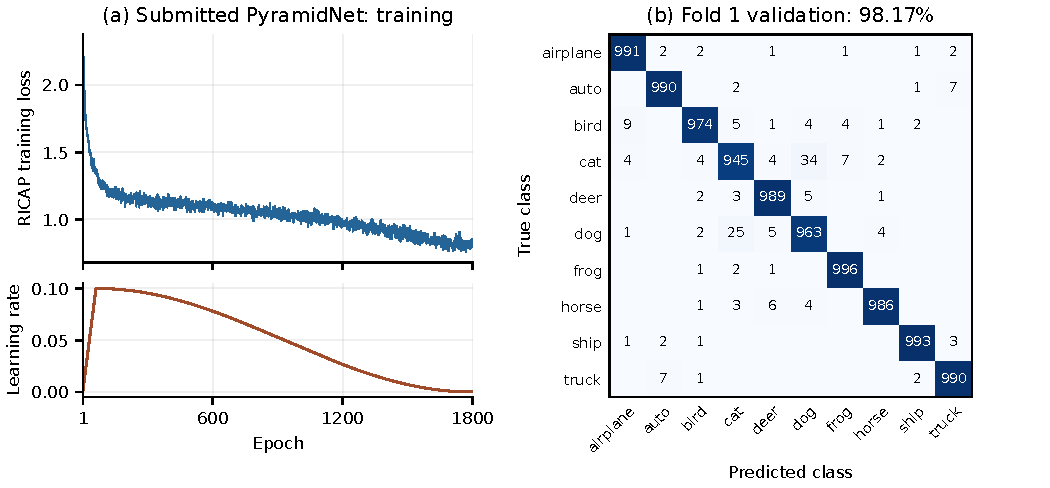
\includegraphics[width=\textwidth]{Figures/pyramid_diagnostics.pdf}
\caption{Diagnostics for the selected 4.80M-parameter PyramidNet. (a) Per-epoch RICAP training loss and learning rate on the 40k training split. (b) Final confusion matrix on the 10k held-out fold, with true classes in rows and predictions in columns. Cells show image counts; color represents the percentage within each true class (1,000 images per row). Validation accuracy is 98.17\%; public competition accuracy is 91.3\%.}
\label{fig:pyramid-diagnostics}
\end{figure*}

\subsection{Classification Performance}
PyramidNet produces the strongest public result among the included submissions (Table~\ref{tab:submissions}). Its 91.3\% accuracy improves on the 600-epoch distilled WRN by 0.7 percentage points while remaining below the five-million-parameter limit. Scratch-distilled SE reaches 91.2\% with 4.685M parameters. These results identify direct PyramidNet training and scratch SE distillation as the strongest submitted recipes in this record. Training-set sizes and validation scope are shown in the table.


Five-fold evaluation shows that the SE recipe's local advantage over distilled WRN is consistent across the available partition (Table~\ref{tab:cv}). SE obtains 97.968\% out-of-fold accuracy, compared with 97.580\% for WRN. It corrects 625 WRN errors and introduces 431, a net improvement of 194 images. The comparison evaluates complete recipes, including their augmentation, training length, and inference settings.

\begin{table}[tb]
\centering\small
\begin{tabular}{lrr}
\toprule
Fold & Distilled WRN & SE-ResNet/RICAP\\
\midrule
0 & 97.36 & 97.80\\
1 & 97.67 & 97.94\\
2 & 97.74 & 97.92\\
3 & 97.54 & 97.99\\
4 & 97.59 & 98.19\\
\midrule
OOF & 97.580 & 97.968\\
\bottomrule
\end{tabular}
\caption{Five-fold development accuracy (\%). WRN: 600 epochs, EMA, plain inference. SE: 1,800 epochs, raw weights, FP32 flip inference.}
\label{tab:cv}
\end{table}

With the augmentation and training schedule matched, PyramidNet improves over SE on both evaluated folds (Table~\ref{tab:pyramid}). Mean accuracy increases from 97.870\% to 98.075\%, with 190 errors corrected and 149 introduced across 20,000 held-out predictions. This supports selecting the gradually widening, ShakeDrop-regularized architecture under the chosen training recipe. Fold 1 had the higher development accuracy and was selected for submission; that checkpoint yielded 91.3\% publicly.

\begin{table}[tb]
\centering\small
\begin{tabular}{lrrrr}
\toprule
Model & Params (M) & Fold 0 & Fold 1 & Mean\\
\midrule
SE164-w22 & 4.685 & 97.80 & 97.94 & 97.870\\
Pyramid110 & 4.805 & 97.98 & 98.17 & 98.075\\
\bottomrule
\end{tabular}
\caption{Matched two-fold architecture comparison (\%). Each network trains for 1,800 epochs on the same 40,000 images within a fold.}
\label{tab:pyramid}
\end{table}

\subsection{Independent Recipe and Ensemble Comparisons}
The independent WRN pipeline improves from 87.9\% to 88.5\% public accuracy after the recipe revision, and its distilled model reaches 88.8\% (Table~\ref{tab:team-results}). SE-ResNet width16 produces 89.4\% and 89.9\% in two runs; width22 produces 90.2\% and 89.6\%. The width22 mean is 0.25 points higher, while its two runs differ by 0.6 points. The two width16 runs disagree on 123 of the 2,000 competition images.

\begin{table*}[t]
\centering\small
\begin{tabular}{llrr}
\toprule
Configuration & Prediction model(s) & Local (\%) & Public (\%)\\
\midrule
WRN-22, initial recipe, 300 epochs, 47.5k train & Single & 97.00 & 87.9\\
Same checkpoint, ten-view TTA & Single & 96.76 & 87.3\\
WRN, revised recipe, 300 epochs, full50k & Single & -- & 88.5\\
WRN, revised recipe, 1,200 epochs, full50k & Single & -- & 88.4\\
Distilled WRN & Single & -- & 88.8\\
SE164 width16, 600 epochs, run 1 & Single & -- & 89.4\\
SE164 width16, 600 epochs, run 2 & Single & -- & 89.9\\
SE164 width22, 600 epochs, run 1 & Single & -- & 90.2\\
SE164 width22, 600 epochs, run 2 & Single & -- & 89.6\\
Two width16 SE runs averaged & Two; 4,976,756 parameters total & -- & 90.2\\
\midrule
Two revised-recipe WRN runs & Two-model average & -- & 88.6\\
Four distilled WRN students & Four-model average & -- & 89.1\\
Four distilled students weighted $3\times$, plus two runs & Six-model average & -- & 89.4\\
Four WRN-22 plus eight WRN-16 & Twelve-model average & -- & 90.3\\
Twelve-model average plus a teammate's hard labels & Twelve models plus votes & -- & 90.1\\
\bottomrule
\end{tabular}
\caption{Public results from the team's initial pipeline. The first two local scores use the 2.5k held-out split with flip and ten-view inference, respectively; other local entries were not retained in that record. Every multi-network entry below the separator exceeds 5M parameters; the two-SE average above it totals 4,976,756.}
\label{tab:team-results}
\end{table*}

Prediction averaging improves this initial pipeline from 88.8\% for the strongest distilled member to 89.1\% with four students, 89.4\% with six weighted members, and 90.3\% with twelve members. The twelve networks span three architecture/recipe variants. Combining them with a teammate's hard-label votes gives 90.1\% at both tested weights. Averaging two width16 SE networks yields 90.2\% with 4,976,756 total parameters. Greedy weight averaging did not improve on the best member and selected a single checkpoint in the tested runs. In comparison, the team's selected single PyramidNet reaches 91.3\%.

\begin{figure*}[t]
\centering
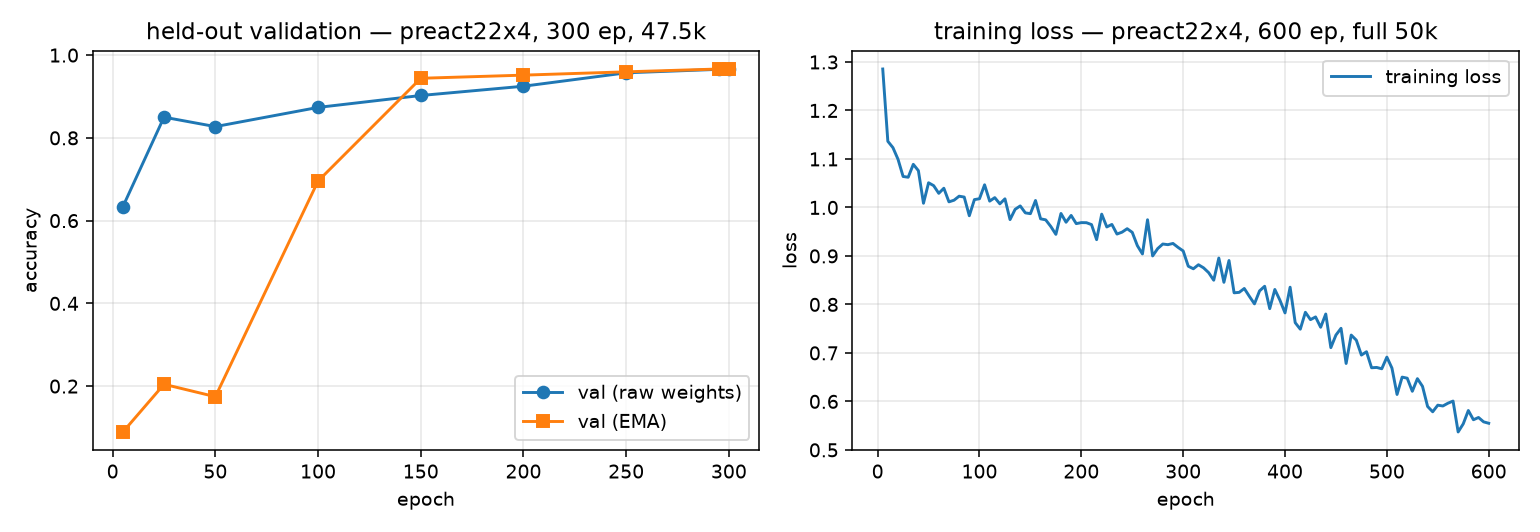
\includegraphics[width=\textwidth]{Figures/training_curves.png}
\caption{Initial-pipeline training curves. Left: nine retained validation measurements, raw and EMA, from the 300-epoch 47.5k/2.5k WRN run; lines connect the recorded points. Right: 120 logged training-loss measurements from the 600-epoch full50k run.}
\label{fig:training}
\end{figure*}

\begin{figure}[!htbp]
\centering
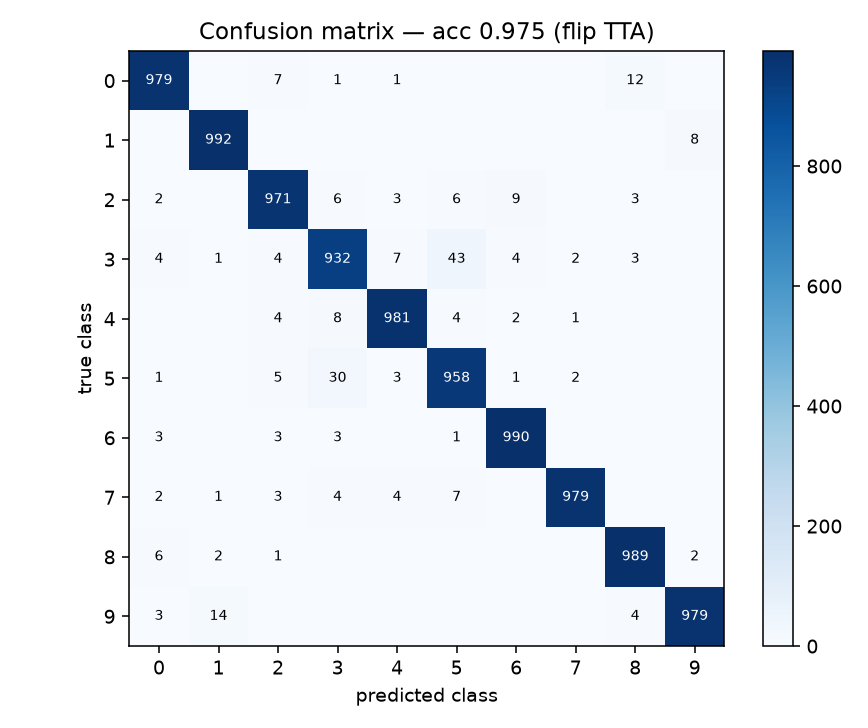
\includegraphics[width=\columnwidth]{Figures/confusion_matrix.png}
\caption{Initial-pipeline WRN-22 confusion matrix on the official 10k CIFAR-10 test split with flip inference (97.50\% accuracy).}
\label{fig:confusion}
\end{figure}

\subsection{Effects of Training and Inference}
\paragraph{Validation ranking.}
On the same fold-0 holdout, scratch SE distillation reaches 98.13\% and SE with SAM reaches 98.20\%, while their public scores are 91.2\% and 90.8\%, respectively. These are the submitted raw KD and EMA SAM weights. The 98.32\% SE result in Table~\ref{tab:submissions} uses the earlier 5k split and is reported separately from these 10k-fold comparisons. The public partition contains approximately 1,000 images, so 0.1 percentage point corresponds to about one image.

\paragraph{Full-data retraining.}
Increasing PyramidNet's training set from 40k to 50k changes 85 of the 2,000 competition predictions and yields 91.2\% public accuracy, compared with 91.3\% for the fold-1 model. The difference is approximately one image on the public partition. Full-data retraining uses the additional 10k images for fitting, so the submitted weights no longer have a held-out fold.

\paragraph{Scratch versus continuation distillation.}
On fold 0, SE/RICAP reaches 97.80\%, a 200-epoch three-teacher KD continuation reaches 98.01\%, and scratch KD reaches 98.13\%. Scratch KD corrects 93 original-SE errors and introduces 60, and its exact checkpoint scores 91.2\% publicly. On this fold, scratch distillation scores higher than both direct SE training and KD continuation. For PyramidNet, a 200-epoch KD continuation with the same three teacher architectures, $T=4$, and $\lambda=0.5$ changes fold-0 accuracy from 97.98\% to 98.01\% but fold-1 accuracy from 98.17\% to 98.00\%. Its mean falls from 98.075\% to 98.005\%. The second fold reveals that the initial local gain does not persist, supporting direct training for the selected PyramidNet.

\paragraph{Alternative regularization.}
The 4.561M-parameter Shake-Shake configuration completes 1,800 epochs, achieves 97.54\% local accuracy, and scores 88.1\% publicly. A separate 200-epoch continuation comparison starts from the 1,800-epoch, 2.49M SE/RICAP model on the original 45k/5k split, distinct from the 600-epoch SE runs in Table~\ref{tab:team-results}. It changes the source model's 98.10\% accuracy to 98.00\% with SGD, 98.20\% with SAM, and 96.38\% with stochastic weight averaging \cite{izmailov2018averaging}. This SAM continuation uses $\rho=0.05$ and raw weights; the scratch SAM row in Table~\ref{tab:submissions} uses width 22, $\rho=0.1$, and EMA. SWA recalibrates BatchNorm on training images after averaging.

\paragraph{Training length and teacher choice.}
Extending the revised WRN recipe from 300 to 1,200 epochs changes public accuracy from 88.5\% to 88.4\%. The independent distillation comparison improves public accuracy from 88.5\% to 88.8\%. In the separate 600-epoch SE comparison, widening from 2.49M to 4.68M parameters changes the two-run mean from 89.65\% to 89.90\%; the measured epoch times are 59 and 58 seconds, respectively.

\paragraph{Additional inference views.}
Ten-view inference using shifted crops and flips reduces the initial WRN's public accuracy from 87.9\% to 87.3\%, with local accuracy changing from 97.00\% to 96.76\%. The selected inference uses horizontal flips. One possible explanation is that shifted crops remove useful border information at $32\times32$ resolution. Two earlier WRN models also reverse their ranking across evaluation sets: official CIFAR-10 accuracy is 97.13\% versus 97.16\%, CIFAR-10.1 accuracy is 92.90\% versus 92.85\%, and public accuracy is 87.9\% versus 88.5\%. The labeled-benchmark accuracies of these two models differ by at most 0.05 percentage points.

\subsection{Robustness and Error Analysis}
Scratch distillation changes which input variations the SE model handles well. On identical fold-0 images (Table~\ref{tab:robust}), its clean accuracy increases by 0.33 points, JPEG accuracy by 3.05 points, and noise accuracy by 2.32 points. Blur accuracy decreases by 7.89 points. The clean gain therefore coexists with a substantial change in sensitivity to image degradation. The perturbation results measure sensitivity beyond clean accuracy; the tested transformations are synthetic.

\begin{table}[tb]
\centering\small
\begin{tabular}{lrr}
\toprule
Condition & SE/RICAP & Scratch-KD SE\\
\midrule
Clean & 97.80 & 98.13\\
Gaussian blur, radius 1 & 91.89 & 84.00\\
JPEG quality 50 & 80.20 & 83.25\\
Gaussian noise, $\sigma=8/255$ & 90.40 & 92.72\\
Resize to 24, then back to 32 & 96.00 & 96.32\\
Contrast $\times0.6$ & 97.74 & 97.95\\
\bottomrule
\end{tabular}
\caption{Fold-0 FP32-flip accuracy (\%) on clean and perturbed validation images.}
\label{tab:robust}
\end{table}

The selected PyramidNet's validation errors concentrate in animal categories. On fold 1, cat accuracy is 94.5\% and dog accuracy is 96.3\%, corresponding to 55 and 37 errors. Together, these categories account for 92 of 183 errors, or 50.3\%, despite representing 20\% of the balanced fold.

Figure~\ref{fig:pyramid-diagnostics} shows the selected model's complete training-loss trajectory, learning-rate schedule, and final validation confusion matrix. The 1,800-epoch run evaluates the held-out fold at the end of training. Its final raw weights give 9,817 correct predictions on 10,000 validation images with FP32 horizontal-flip inference; these are the same weights used for the 91.3\% public submission.


A separate check tests whether preprocessing or export changes explain the validation--public discrepancy. The loader checks file paths, sample IDs, and label ranges. Replaying the selected PyramidNet through the submission pipeline on lossless PNG exports of its 10k held-out images reproduces 98.17\% with zero label changes. Normalized input tensors match exactly, and the largest probability difference across evaluation batch sizes is $1.43\times10^{-6}$. The checked loading and export path preserves all validation predictions. The 6.87-point gap between local and public accuracy remains, with development-set selection and evaluation-distribution differences as possible contributors whose individual effects are unmeasured.

\subsection{Initial-Pipeline Diagnostics and Reproducibility}
The initial pipeline's executed notebook provides the training curves in Figure~\ref{fig:training} and the confusion matrix in Figure~\ref{fig:confusion}. Both initial-pipeline figures use the 600-epoch, full-50k WRN-22 run \texttt{arch\_preact22x4\_s0} for their full-data measurements; the validation curve comes from the separate 300-epoch holdout run. This WRN-22 checkpoint has 4,326,986 parameters and reaches 97.50\% on the official 10k CIFAR-10 test split with flips, compared with 97.32\% under plain inference. Per-class recall ranges from 93.2\% for cats to 99.2\% for automobiles. These benchmark measurements accompany the development-fold and competition results as distinct evaluations.



The selected-model notebook, \texttt{proj1/report\_results.ipynb}, prints the recomputed parameter count, accuracy from retained validation predictions, and public score from the submission receipt. Training and CSV inference use \texttt{proj1/train.py} and \texttt{proj1/predict.py}, with commands in the project README. The initial pipeline has a separate executed notebook. The selected PyramidNet retains its configuration, split indices, checkpoint, per-image probabilities, and submission receipt. The team also used in-memory image buffering and GPU tensor augmentations to reduce repeated file access in an alternative training pipeline.

\subsection{Design Trade-offs}
SE supplies a compact 2.49M-parameter option; increasing its width to 22 uses 4.68M parameters and changes the initial pipeline's two-run public mean from 89.65\% to 89.90\%. PyramidNet allocates 4.80M parameters through gradual widening and parameter-free shortcut adjustments, and gives the higher accuracy in both matched architecture comparisons. Distillation increases training-time computation while retaining a single student at inference; its 0.33-point clean-accuracy gain for SE accompanies different sensitivities to blur, compression, and noise. These comparisons motivate evaluating architecture, training recipe, and robustness together when choosing a compact classifier.

\subsection{Inference Parameter Budget}
The selected classifier is a single 4,804,512-parameter PyramidNet. The twelve-network average contains roughly 52--57M trainable parameters, exceeding the five-million limit when counted as one inference system. Two width16 SE networks total 4,976,756 parameters and score 90.2\%. The selected 91.3\% result uses one network and horizontal-flip averaging. Teacher networks contribute only during distillation training.

\section{Conclusion}
The selected PyramidNet combines gradual channel growth, ShakeDrop, and image augmentation to reach 91.3\% public accuracy with 4.80M parameters. The SE recipe scores higher than distilled WRN on all five development folds, and PyramidNet scores higher than SE on two matched folds. Scratch SE distillation provides another compact single-model result at 91.2\%. The comparisons also distinguish where training changes help: scratch distillation improves clean SE accuracy, SAM improves SE on its development fold, and prediction averaging improves the initial WRN pipeline. The final classifier uses one PyramidNet with horizontal-flip inference.

\bibliography{project1}
\end{document}
